\documentclass{article}
\usepackage[utf8]{inputenc}
\usepackage{natbib}
\usepackage{graphicx}
\usepackage{geometry}
\usepackage{color}
\usepackage{float}
\usepackage{hyperref}
\usepackage{enumerate}
\usepackage{fancyhdr}
\usepackage{titling}
\usepackage{amsmath}
\usepackage{amsmath,amssymb,amsthm}
\usepackage{listings}
\usepackage[table,xcdraw]{xcolor}
\usepackage{ulem} 
\usepackage{graphicx}
\renewcommand{\baselinestretch}{1.2}%Adjust Line Spacing
\newtheorem{Q}{Question}
\geometry{left=2.5cm,right=2.5cm,top=2.5cm,bottom=2.5cm}% Adjust Margins of the File
\usepackage{tikz-qtree}
\usetikzlibrary{graphs}
\tikzset{every tree node/.style={minimum width=2em,draw,circle},
	blank/.style={draw=none},
	edge from parent/.style=
	{draw,edge from parent path={(\tikzparentnode) -- (\tikzchildnode)}},
	level distance=1.2cm}
\setlength{\droptitle}{-6em}
%%% Code style
\lstset{
	%backgroundcolor=\color{red!50!green!50!blue!50},%代码块背景色为浅灰色
	rulesepcolor= \color{gray}, %代码块边框颜色
	breaklines=true,  %代码过长则换行
	numbers=left, %行号在左侧显示
	numberstyle= \small,%行号字体
	keywordstyle= \color{magenta},%关键字颜色
	commentstyle=\color{blue}, %注释颜色
	frame=shadowbox, %用方框框住代码块
	tabsize=3, %缩进大小
	showspaces = false
}
% Create horizontal rule command with an argument of height
\newcommand{\horrule}[1]{\rule{\linewidth}{#1}}
% Set the title here
\title{
    \normalfont \normalsize
    \textsc{ShanghaiTech University} \\ [25pt]
    \horrule{0.5pt} \\[0.4cm] % Thin top horizontal rule
    \huge CS101 Algorithms and Data Structures\\ % The assignment title
    \LARGE Fall 2019\\
    \LARGE Homework 7\\
    \horrule{2pt} \\[0.5cm] % Thick bottom horizontal rule
}
% wrong usage of \author, never mind
\author{}
\date{Due date: 23:59, November 10, 2019}

% set the header and footer
\pagestyle{fancy}
\lhead{CS101 Algorithms and Data Structures}
\chead{Homework 6}
\rhead{Due date: 23:59, November 3, 2019}
\cfoot{\thepage}
\renewcommand{\headrulewidth}{0.4pt}

% special settings for the first page
\fancypagestyle{firstpage}
{
	\renewcommand{\headrulewidth}{0pt}
	\fancyhf{}
	\fancyfoot[C]{\thepage}
}

% Add the support for auto numbering
% use \problem{title} or \problem[number]{title} to add a new problem
% also \subproblem is supported, just use it like \subsection
\newcounter{ProblemCounter}
\newcounter{oldvalue}
\newcommand{\problem}[2][-1]{
	\setcounter{oldvalue}{\value{secnumdepth}}
	\setcounter{secnumdepth}{0}
	\ifnum#1>0
		\setcounter{ProblemCounter}{#1}
	\else
		\stepcounter{ProblemCounter}
	\fi
	\section{Problem \arabic{ProblemCounter}: #2}
	\setcounter{secnumdepth}{\value{oldvalue}}
}
\newcommand{\subproblem}[1]{
	\setcounter{oldvalue}{\value{section}}
	\setcounter{section}{\value{ProblemCounter}}
	\subsection{#1}
	\setcounter{section}{\value{oldvalue}}
}

\begin{document}
\maketitle
\thispagestyle{firstpage}
%\newpage
\vspace{3ex}

\begin{enumerate}
\item Please write your solutions in English. 

\item Submit your solutions to gradescope.com.  

\item Set your FULL Name to your Chinese name and your STUDENT ID correctly in Account Settings. 

\item If you want to submit a handwritten version, scan it clearly. Camscanner is recommended. 

\item When submitting, match your solutions to the according problem numbers correctly. 

\item No late submission will be accepted.

\item Violations to any of above may result in zero score. 
\end{enumerate}
\newpage

\section{(3') Minimum Spanning Tree and Topological Sort}
Each question has one or more correct answer(s). Select all the correct answer(s). For each question, you get $0$ point if you select one or more wrong answers, but you get $0.5$ point if you select a non-empty subset of the correct answers.\\
\textit{Note that you should write you answers of section 1 in the table below.}
\begin{table}[htbp]
	\begin{tabular}{|p{2cm}|p{2cm}|p{2cm}|}
		\hline 
		Question 1 & Question 2 & Question 3  \\ 
		\hline 
		\textbf{CD} &\textbf{D}  &\textbf{AD}   \\ 
		\hline 
	\end{tabular} 
\end{table}
\begin{Q}
Topological Sort can be carried out on what kinds of graphs:
\begin{enumerate}[(A)]
	\item All weight acyclic graphs
	\item All directed graphs
	\item All (Directed) Trees
	\item All unweight directed acyclic graphs
	\item All cyclic directed graphs
\end{enumerate}
\end{Q}


\iffalse
\begin{Q}
Suppose we are given a directed graph $G(V,E)$ in which every edge has a distinct positive edge weight. Suppose that we want to compute the maximum-weight acyclic subgraph of $G$ (where the weight of a subgraph is the sum of its edges’ weights). Assume that $G$ is weakly connected, meaning that there is no cut with no edges crossing it in either direction.\\
Here is an analog of Prim’s algorithm for directed graphs. Start from an arbitrary vertex $s$, initialize $S=\{s\}$ and $F=\emptyset$. While $S\neq V$, find the maximum-weight edge $(\mu,v)$ with one endpoint in $S$ and one endpoint in $V-S$. Add this edge to $F$, and add the appropriate endpoint to $S$.\\
Here is an analog of Kruskal’s algorithm. Sort the edges from highest to lowest weight. Initialize $F=\emptyset$. Scan through the edges; at each iteration, add the current edge $i$ to $F$ if and only if it does not create a directed cycle.\\
Which of the following is true?
\begin{enumerate}[(A)]
	\item Both algorithms might fail to compute a maximum-weight acyclic subgraph. 
	\item Only the modification of Kruskal’s algorithm always computes a maximum-weight acyclic subgraph.
	\item Only the modification of Prim’s algorithm always computes a maximum-weight acyclic subgraph.
	\item Both algorithms always compute a maximum-weight acyclic subgraph.
\end{enumerate} 
\end{Q}

\fi
\begin{Q}
	Consider the following algorithm that attempts to compute a minimum spanning tree of a connected undirected graph $G$ with distinct edge costs. First, sort the edges in decreasing cost order (i.e., the opposite of Kruskal’s algorithm). Initialize $T$ to be all edges of $G$. Scan through the edges (in the sorted order), and remove the current edge from $T$ if and only if it lies on a cycle of $T$.\\	
	Which of the following statements is true?
	\begin{enumerate}[(A)]
		\item The output of the algorithm will never have a cycle, but it might not be connected.
		\item The algorithm always outputs a spanning tree, but it might not be a minimum cost spanning tree.
		\item The output of the algorithm will always be connected, but it might have cycles.
		\item The algorithm always outputs a minimum spanning tree.
	\end{enumerate} 
\end{Q}


\begin{Q}
	You are given a connected undirected graph $G$ with distinct edge costs, in adjacency list representation. You are also given the edges of a minimum spanning tree $T$ of $G$. This question asks how quickly you can recompute the MST if we change the cost of a single edge. Which of the following are true? [RECALL: It is not known how to deterministically compute an MST from scratch in $O(m)$ time, where $m$ is the number of edges of $G$.]
	
	\begin{enumerate}[(A)]
		\item Suppose $e\in T$ and we increase the cost of $e$. Then, the new MST can be recomputed in $O(m)$ deterministic time.
		\item Suppose $e\notin T$ and we increase the cost of $e$. Then, the new MST can be recomputed in $O(m)$ deterministic time.
		\item Suppose $e\in T$ and we decrease the cost of $e$. Then, the new MST can be recomputed in $O(m)$ deterministic time.
		\item Suppose $e\notin T$ and we decrease the cost of $e$. Then, the new MST can be recomputed in $O(m)$ deterministic time.
	\end{enumerate} 
\end{Q}


\pagebreak


\section{(4')True or False}
The following statements may or may not be correct. In each case, give a counterexample (if it isn’t correct). Always assume that the graph $G = (V, E)$ is undirected. Do not assume that edge weights are distinct unless this is specifically stated.
\begin{itemize}
	\item If graph $G$ has more than $|V|-1$ edges, and there is a unique heaviest edge, then this edge cannot be part of a minimum spanning tree.
	\par\textbf{Answer:}
	\par\textbf{False.} Consider the following graph:
	\par\begin{tikzpicture}
  [scale=0.5,auto=left,every node/.style={circle, fill=white, draw}]
  \node (n1) at (0,3) {A};
  \node (n2) at (3,6) {B};
  \node (n3) at (6,3) {C};
  \node (n4) at (3,0) {D};
  \node (n5) at (12,3) {E};
  \foreach \from/\to in {n1/n2,n2/n3,n1/n4,n3/n4,n3/n5}
    \draw (\from) -- (\to);
    \end{tikzpicture}
    \par Even if the edge $C-E$ is the heaviest, it must still be part of the MST since it's the only edge between $C$ and $E$ and the MST must contains an edge between those two vertices.
	\vspace{0.3in}
	
	\item If $e$ is part of some MST of $G$, then it must be a lightest edge across some cut of $G$.
	\par\textbf{Answer:}
	\par\textbf{True.} If $e$ is not the lightest edge across some cut of $G$, then there must be another lightest edge $e'$ across the cut of $G$, then $e$ doesn't belong to the MST, which is contradictory. Thus $e$ must be a lightest edge across some cut of $G$.
	\vspace{0.3in}

	\item Prim’s algorithm works correctly when there are negative edges.
	\par\textbf{Answer:}
	\par\textbf{True.} That algorithm always adds the lightest edge between the unfinished MST and other unvisited vertices, negative edges can also be compared with their values so Prim's algorithm works fine with negative edges.
    \vspace{0.3in}
\end{itemize}
\newpage
\section{(18') Minimum Spanning Tree}
Given the following undirected, weighted graph, compute two minimum spanning trees.
\begin{figure}[H]
	\centering
	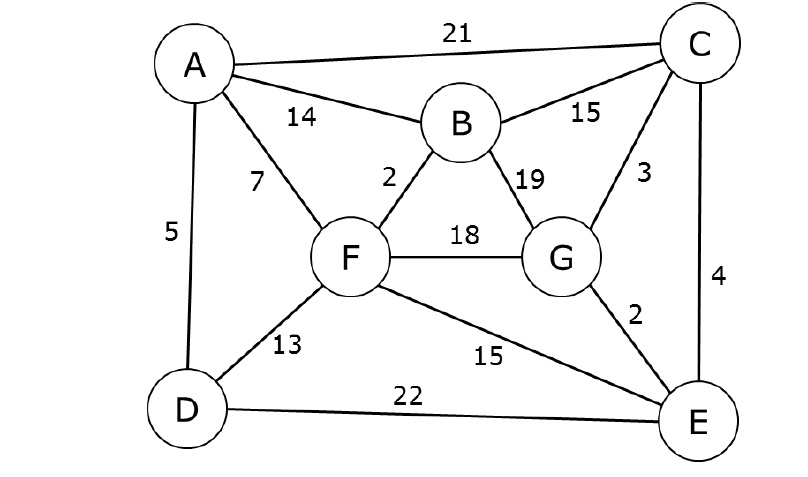
\includegraphics[width=0.6\textwidth]{./mst}
\end{figure}

(1)(5') Step through Prim’s algorithm to calculate a minimum spanning tree starting from vertex \textbf{A}. Show your steps in the table below. As the algorithm proceeds, cross out old values and write in new ones, from left to right in each cell. If during your algorithm two unvisited vertices have the same distance, use alphabetical order to determine which one is selected first. As an example, Row B is filled already.\\
\begin{table}[htbp]
	\begin{tabular}{|p{4cm}|p{4cm}|p{4cm}|}
		\hline 
		\textbf{Vertex} & \textbf{Distance} & \textbf{From(Vertex)}\\ 
		\hline 
		A&- &-  \\
		\hline  
		B&\sout{14} 2 &\sout{A} F \\ 
		\hline 
		C&\sout{21} 15 &\sout{A} B  \\  
		\hline 
		D&5  &A \\
		\hline 
		E&\sout{22} \sout{15} \sout{4} 2 &\sout{D} \sout{F} \sout{C} G  \\ 
		\hline 
		F&7  &A  \\ 
		\hline 
		G&\sout{18} 3  &\sout{F} C \\
		\hline 
	\end{tabular} 
\end{table}
\pagebreak

(2)(2') Draw the MST you get by this algorithm:\\
\par\textbf{Answer:}\\
\par\begin{tikzpicture}[level/.style={sibling distance=60mm/#1},grow=right]
\node [circle,draw] (a){A}
  child {node [circle,draw] (d) {D} edge from parent node[above,right] {5}}
  child {node [circle,draw] (f) {F} 
    child {node [circle,draw] (b) {B}
    	child {node [circle,draw] (c) {C}
    		child {node [circle,draw] (g) {G}
    			child {node [circle, draw] (e) {E} edge from parent node[above] {2}
    					} edge from parent node[above] {3}
    				} edge from parent node[above] {15}
    			} edge from parent node[above] {2}
    		} edge from parent node[below,right] {7}
    	  };
\end{tikzpicture}
\vspace{0.5in}

(3)(9') Step through Kruskal’s algorithm to calculate a minimum spanning tree of the graph. Show your steps in the table below, including the disjoint sets at each iteration. If you can select two edges with the same weight, select the edge that would come alphabetically last (e.g., select E—F before B—C. Also, select A—F before A—B).\\
\begin{table}[htbp]
	\begin{tabular}{|p{4cm}|p{4cm}|p{4cm}|}
		\hline 
		\textbf{Edge Added} & \textbf{Edge Cost} & \textbf{Disjoint Sets}\\ 
		\hline 
		-&- & (A)(B)(C)(D)(E)(F)(G)\\
		\hline  
		E-G&2 &(A)(B)(C)(D)(EG)(F) \\ 
		\hline 
		B-F&2 &(A)(BF)(C)(D)(EG)  \\ 
		\hline 
		C-G&3 &(A)(BF)(CEG)(D)  \\ 
		\hline 
		A-D&5 &(AD)(BF)(CEG) \\
		\hline 
		A-F&7 &(ABDF)(CEG)  \\ 
		\hline 
		E-F&15 &(ABCDEFG)  \\ 
		\hline 
	\end{tabular} 
\end{table}
\pagebreak

(4)(2') Draw the MST you get by this algorithm: \\
\par\textbf{Answer:}\\
\par\begin{tikzpicture}[level/.style={sibling distance=60mm/#1},grow=right]
\node [circle,draw] (e){E}
  child {node [circle,draw] (g) {G}
  	 child {node [circle,draw] (c) {C} edge from parent node[above] {3}
  	       } edge from parent node[above,right] {2} 
  	 	  }
  child {node [circle,draw] (f) {F}
  	 child {node [circle,draw] (b) {B} edge from parent node[above,right] {2}}
  	 child {node [circle,draw] (a) {A}
  	   child {node [circle,draw] (d) {D} edge from parent node[above] {5}
  	        } edge from parent node[below,right] {7}
  	        } edge from parent node[below,right] {15}
  		  };
\end{tikzpicture}

\end{document}